\documentclass[final]{beamer}
\mode<presentation>
  {
  \usetheme{Rutgers}
  }
  \usepackage{amsmath,amsthm, amssymb, latexsym}
  \boldmath
  \usepackage[english]{babel}
  \usepackage[latin1]{inputenc}
  \usepackage{lmodern}
  \usepackage[orientation=portrait,size=a0,scale=1.4,debug]{beamerposter}
  
\usepackage{myalgorithm}
\usepackage{wrapfig}
\usepackage[noend]{myalgorithmic}
\usepackage{multirow}
\usepackage{multicol}
\usepackage{graphicx,wrapfig,lipsum}


  %%%%%%%%%%%%%%%%%%%%%%%%%%%%%%%%%%%%%%%%%%%%%%%%%%%%%%%%%%%%%%%%%%%%%%%%%%%%%%%%%
  \title[Maneuvers]{Learning Efficient Maneuver Sets for Kinodynamic Motion Planning}
  \author[Sivaramakrishnan]{Aravind Sivaramakrishnan, Zakary Littlefield and Kostas E. Bekris}
  \institute[Rutgers]{Department of Computer Science, Rutgers, the State University of New Jersey}



  %%%%%%%%%%%%%%%%%%%%%%%%%%%%%%%%%%%%%%%%%%%%%%%%%%%%%%%%%%%%%%%%%%%%%%%%%%%%%%%%%
  \newlength{\blocklen}
  \begin{document}
  \setlength{\blocklen}{0.49\textwidth}
  \begin{frame}[t]{} 
    \vspace {-0.5in}
    \begin{columns}[t]
	\begin{column}{0.50\textwidth}
		\begin{block}{\large Motivation}
		    \begin{columns}[t]
			    \begin{column}{0.62\textwidth}
					    If a kinodynamic planner $[1]$ has access to local maneuvers that balance an exploitation-exploration trade-off, the planner's per iteration performance is significantly improved.
					    \begin{itemize}
					    	\item Exploitation maneuvers guide the system towards the goal given local heuristic information
					    	\item Exploration maneuvers move the system in different directions so as to deal with situations that the heuristic does not provide good guidance.
					    \end{itemize}
					    % \item These maneuvers can be computed online employing a metric similar to $[2]$, tailored to each state of the robot selected for propagation during planning.
			    \end{column}
			    \begin{column}{0.35\textwidth}
			    	\centering
					\begin{figure}
					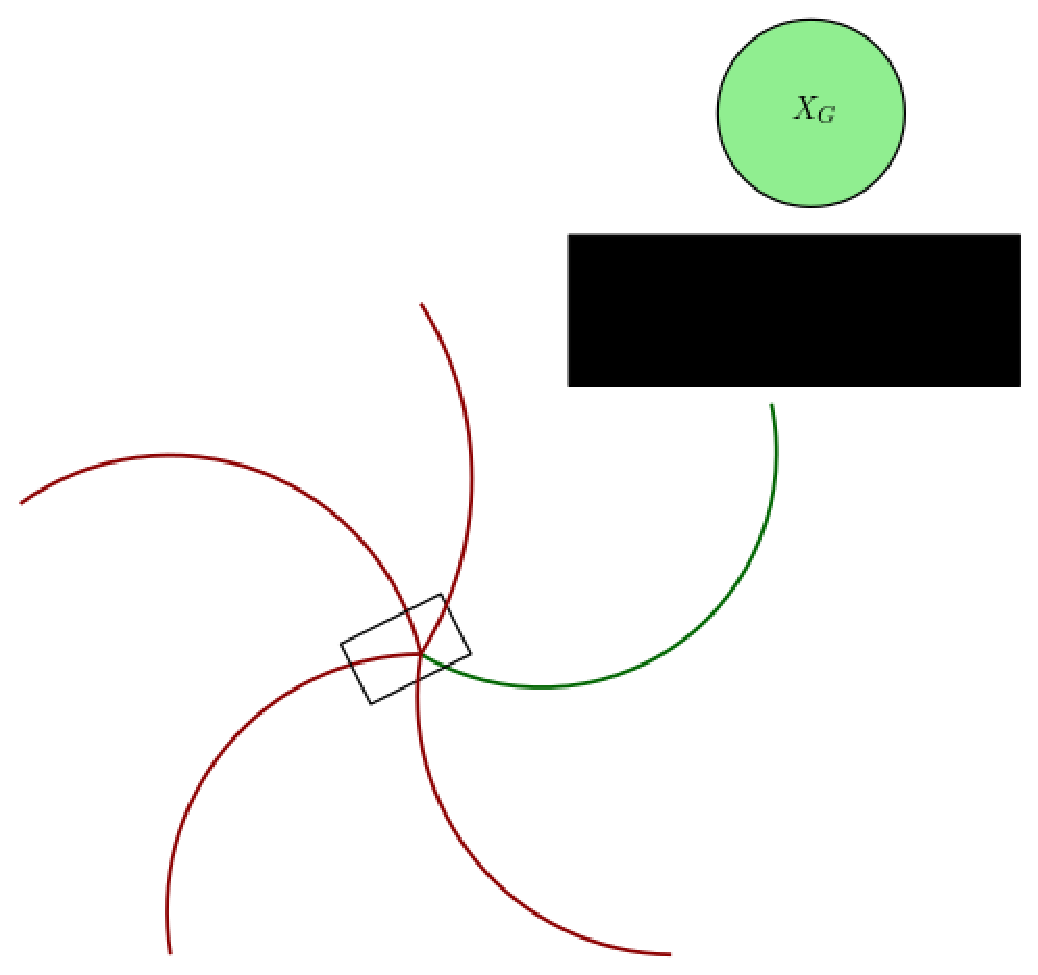
\includegraphics[scale=0.67]{figures/maneuver_sets.eps}
					\caption{Exploitative (green) and Explorative (red) maneuvers for a robot planning to reach $X_G$ (green circle) behind an obstacle (black box). \vspace{-.2in}}
					\end{figure}
			    \end{column}
		    \end{columns}
		\end{block}
	\end{column}
	\begin{column}{0.50\textwidth}
		\begin{block}{\large Motion planning with informed maneuvers}
		    % \centering
		    % 	\begin{figure}[h]
		    % 		\includegraphics[width = 0.75\textwidth, height=2.5in]{meta_items}	\hspace{0.1in}
		    % 		\caption{The 25 APC objects categorized by broad object class}
	    	% 	\end{figure}
	    	% 	\vspace{-0.2in}
		    \begin{columns}[T]
		    	\begin{column}{0.98\textwidth}
					\begin{itemize}
						\item Informed maneuvers can be computed online employing a metric similar to $[2]$, tailored to each state of the robot selected for propagation during planning. \vspace{0.1in}
						\begin{table}[h!]
						\centering
						\begin{tabular}{|l|l|l|l|}
						\hline
						        & \textbf{Iteration} & \textbf{Comp. Time} & \textbf{Path Cost} \\ [0.5ex] \hline
						Random  & 1471                    & 0.2                   & 50.47                  \\ \hline
						Curated & 686                    & 12.15                & 48.13                  \\ \hline
						\end{tabular}
						\caption{First solution statistics between DIRT using random and curated maneuvers.}
						\label{table:Rastar}
						\vspace{0.1in}
					\end{table}
						\item Very effective in finding a high-quality solution in fewer number of iterations but computational becomes prohibitive.
						\item \textbf{Goal:} Develop an approach that achieves the same objective as the curation but can generate the maneuvers fast.
					\end{itemize}
				\end{column}
				% \begin{column}{0.38\textwidth}
				% \includegraphics[height=2.5in]{datacollectionsetup_2}	\hspace{0.1in}
				% \end{column}
			\end{columns}
		\end{block}
	\end{column}
\end{columns}	
		    

    \vfill
    
\begin{columns}[t]
	\begin{column}{0.65\textwidth}
		\begin{block} {\large Input to the learning process}
			\begin{columns}[T]
				\centering
				\begin{column}{0.59\textwidth}
					\begin{itemize}
						\item A regular set of points $\mathbb{X}_{local}$ in the vicinity of $x_0$ are collision checked to generate a binary 2D map $o_{local}$ indicating the presence of obstacles in the workspace.
						\item The heuristic $h(x)$ is also evaluated at each $x \in \mathbb{X}_{local}$, resulting in a 2D matrix $h_{local}$.
					\end{itemize}
				\end{column}
				\begin{column}{0.20\textwidth}
					\centering
					\begin{figure}
					
\includegraphics[width=0.5\columnwidth]{o_example}
					\caption{$o_{local}$} 
					\end{figure}
				\end{column}
				\begin{column}{0.20\textwidth}
					\centering
					\begin{figure}
					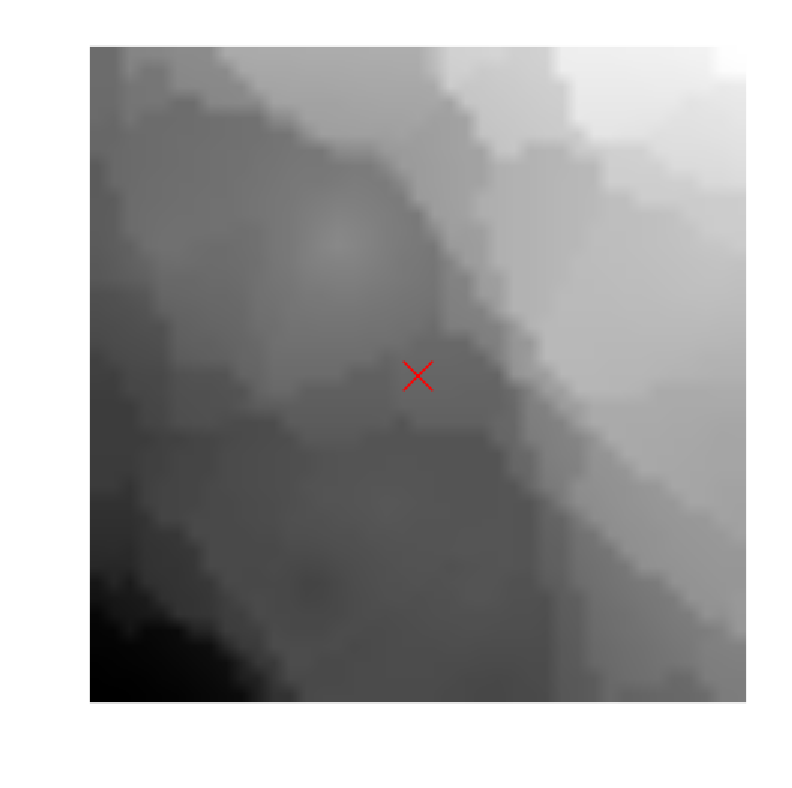
\includegraphics[width=0.5\columnwidth]{h_example}
					\caption{$h_{local}$} 
					\end{figure}
					\vspace{0.1in}
				\end{column}
			\end{columns}
		\vspace{-0.4in}
		\end{block}
		\begin{block}{\large Proposed architecture}
			\begin{itemize}
			\item Multi-layered neural networks $F_x, F_o, F_h$ act on the inputs to produce $x_0^*, o_{local}^*, h_{local}^*$. 
			\item An operator $M_0(x_0^*, o_{local}^*,h_{local}^*)$ produces feature vector  $x_f^0$.
			\item Exploitative control $u^0$ is obtained as $u^0 = F^0(x_f^0)$, where $F^0$ is also a neural network.
			\item Remaining $N$ exploratory controls are obtained as follows.
			\vspace{-.1in}
			\begin{align*}
				x_f^k &= M_k(x_f^0,U_{k-1}) \\
				u^{k} &= F^k(x_f^k) 
			\end{align*}
			\vspace{-.1in}
			where for all $k \geq 1$, $U_k = \{u^0,u^1,..,u^{k-1}\}$. For the exploitative control ($k=0$), $U_{k-1}$ is the empty set.
			\vspace{0.1in}
			\end{itemize}			
			\begin{figure}[h!]
				\centering
				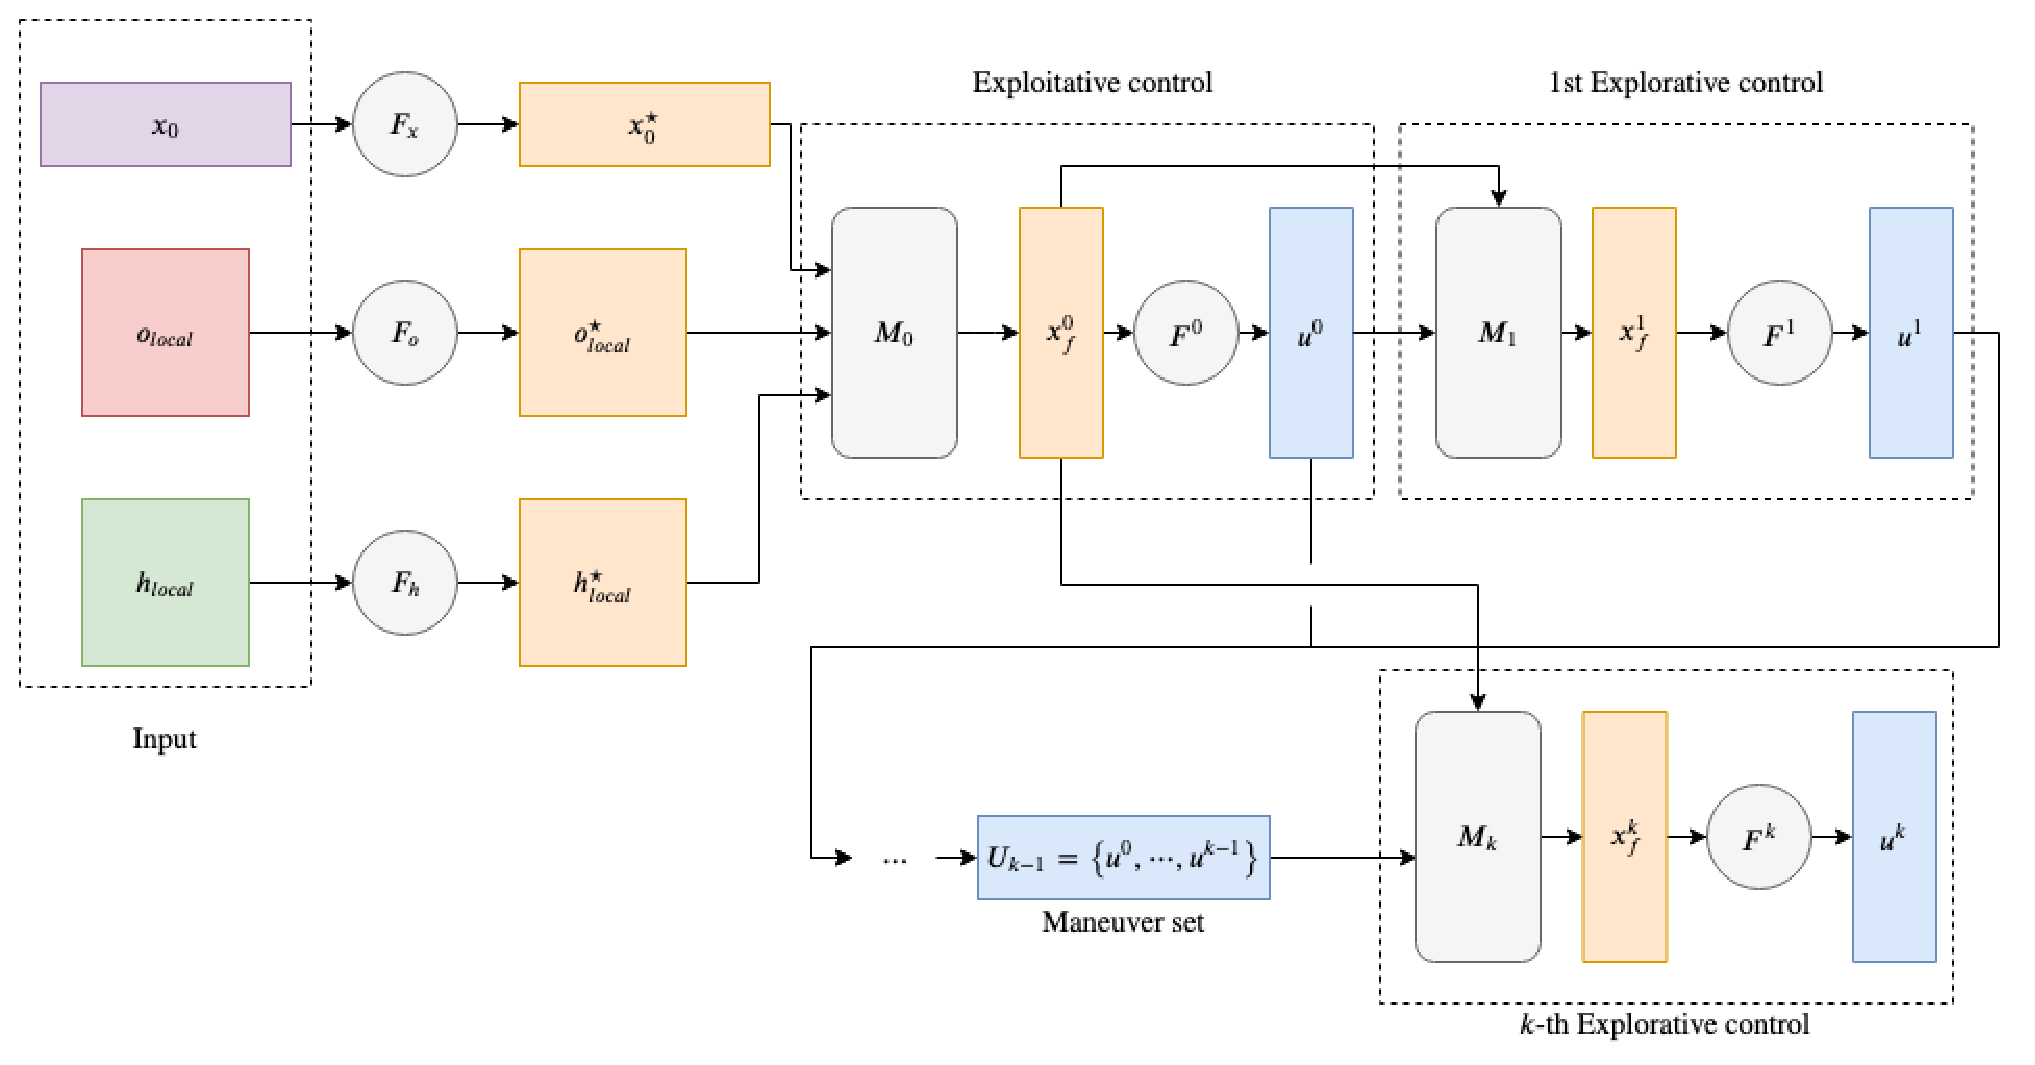
\includegraphics[scale=0.95]{cgraph}
				\vspace{-.1in}
				\caption{Computation graph of $U_k = \hat{f}(x_0,o_{local},h_{local})$. For $k=N, U_k = \hat{U} = \{u^0,\cdots,u^N\}$.\vspace{-.15in}}
				\label{fig:cgraph}
			\end{figure}
			\vspace{-.1in}
		\end{block}
	\end{column}
	\begin{column} {0.35\textwidth}
		\begin{block}{\large Experimental Setup}
		\begin{figure}[h!]
			\centering
			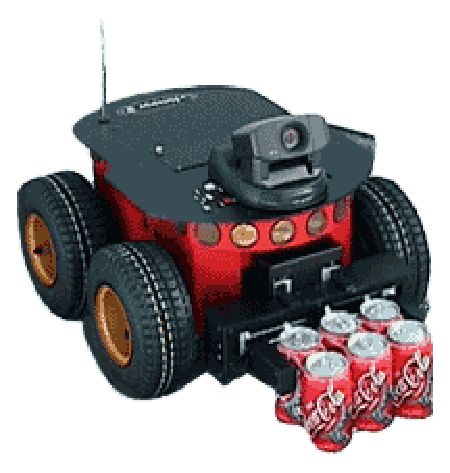
\includegraphics[scale=0.75]{skid-steer}
			\vspace{-.1in}
			\caption{Treaded vehicle with 5 dim. state space (SE(2) augmented by steering angle and forward velocity) and 2 dim. control space (acceleration of left and right treads) used in our experiments.}
		\end{figure}
		\begin{itemize}
			\item Randomly place obstacles in the workspace so they cover one-third of the reachable workspace. 
			\item Execute the DIRT planner $[1]$ with the online curation procedure on multiple problem instances in such workspaces. 
			\item Euclidean distance to the goal in the workspace is used as the heuristic function. %The cost is the duration of the solution trajectory.
			\item For each node $x_0$ the planner selects to propagate, store $o_{local}$ and $h_{local}$ maps, and maneuver set $\hat{U}$ of size 5 curated from 1000 randomly sampled maneuvers.
			\item Train two networks - fully connected (\texttt{FC}) and convolutional (\texttt{Conv})
		\end{itemize}
		\centering
			\vspace{0.2in}
			\begin{columns}
				\centering
				\begin{column}{0.4\columnwidth} 
					\centering
					\begin{figure}
					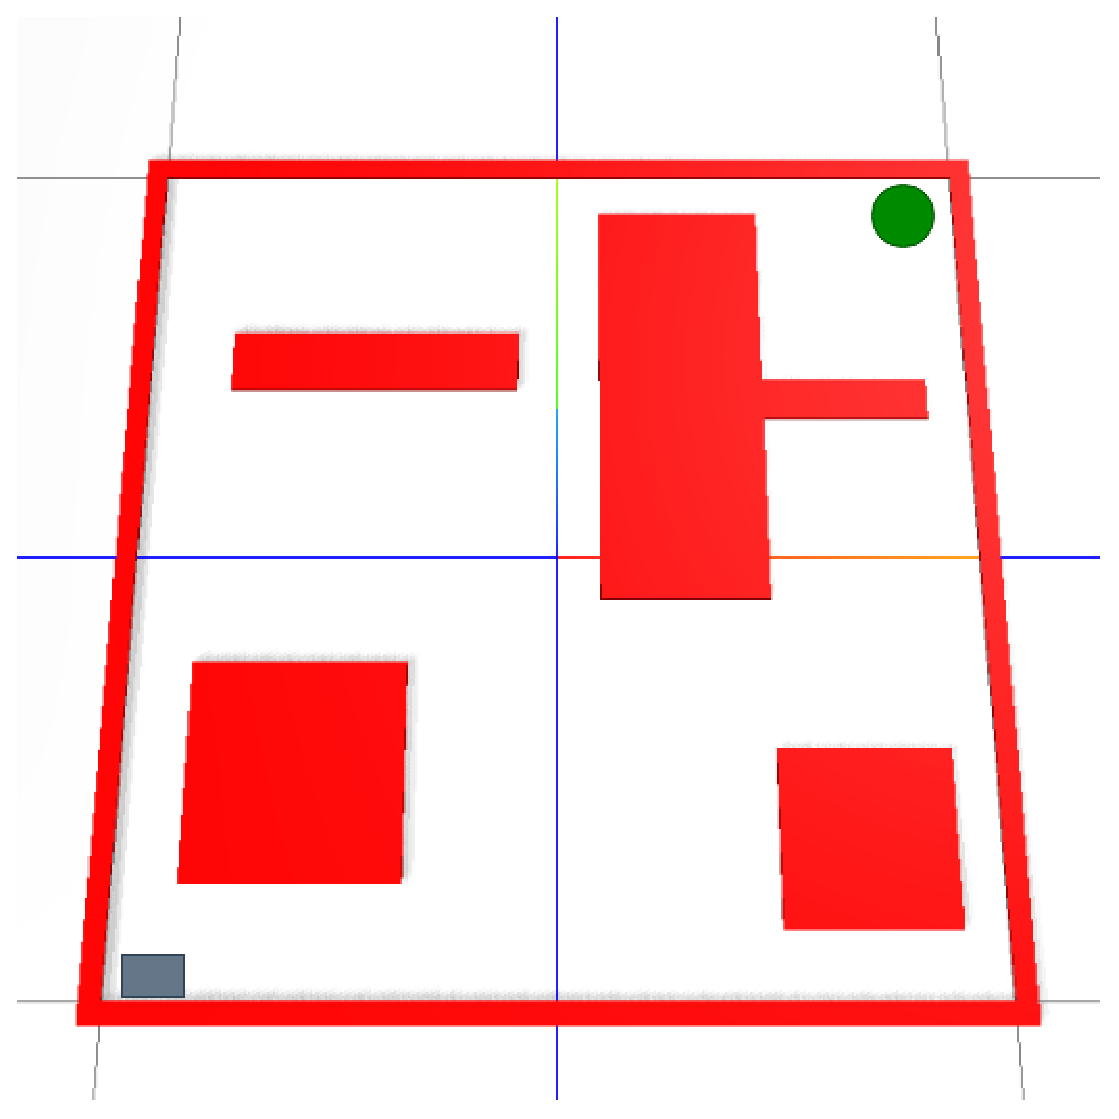
\includegraphics[scale=0.5]{iai}
					\caption{\texttt{Greedy}} 
					\end{figure}
				\end{column}
				\hfill
				\begin{column}{0.4\columnwidth} 
					\centering
					\begin{figure}
					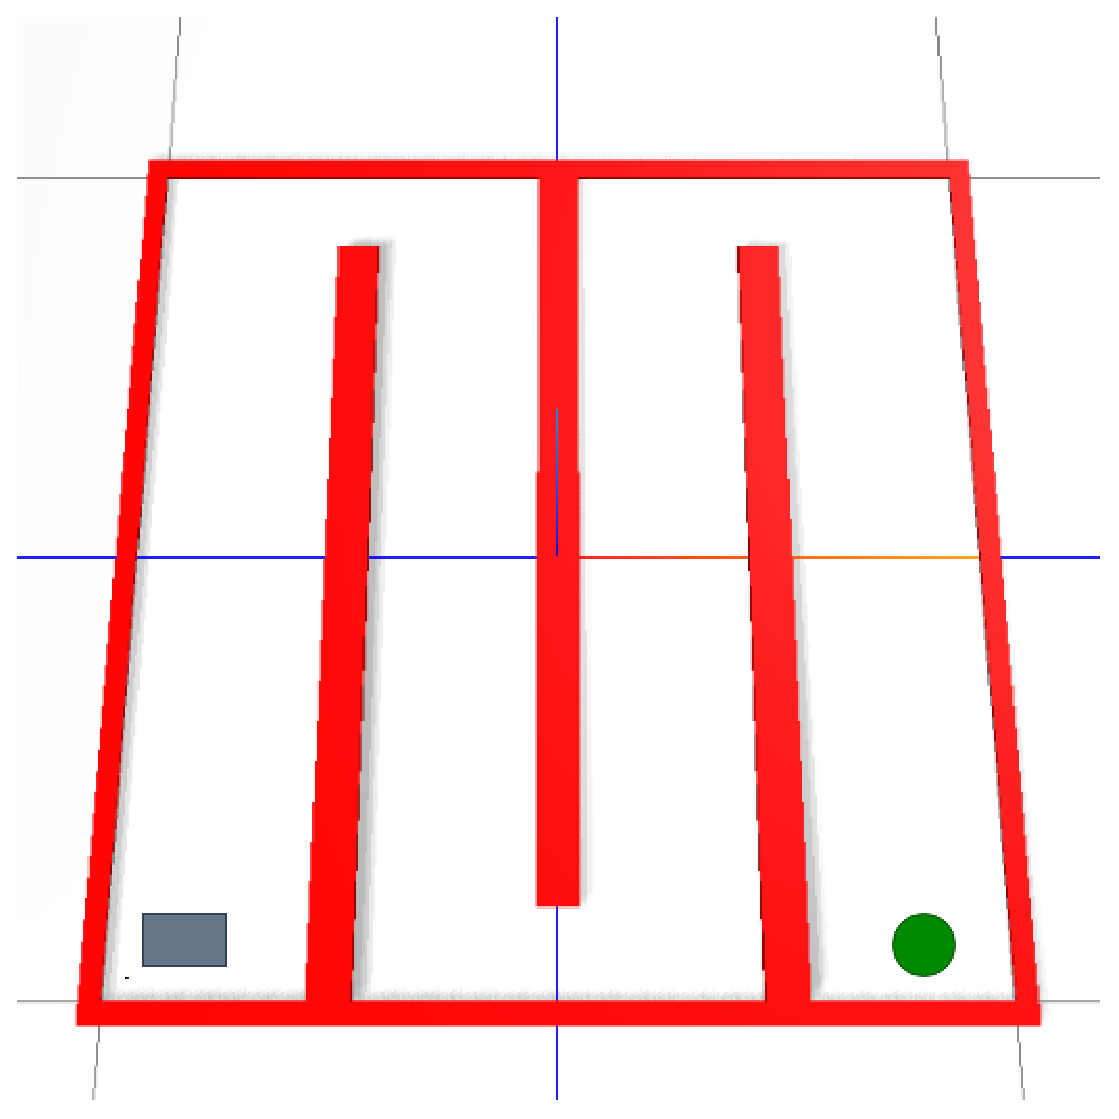
\includegraphics[scale=0.5]{flappy}
					\caption{\texttt{Explore}} 
					\end{figure}
				\end{column}
			\end{columns}
			\vspace{0.2in}
			\small{Environments: The grey rectangle is the starting pose of the robot (facing right) and the green circle is the goal region. The robot must avoid the red obstacles.}
			\vspace{0.1in}
		\end{block}
	\end{column}
\end{columns}




    \vfill
    \begin{columns}[t]
	\begin{column}{0.68\textwidth}
	\vspace{-0.1in}
		\begin{block}{\large Solution statistics}
		We compare the performance of DIRT (after 50k iterations) for the following maneuvers: 
		\begin{itemize}
			\item random (DIRT - Random) 
			\item only exploitative control predicted by the network (DIRT - FC (Exploit), DIRT - Conv (Exploit))
			\item both exploitative and explorative controls are predicted by the networks ((DIRT - FC (All), DIRT - Conv (All))
		\end{itemize} 
			\vspace{0.1in}
			\begin{table}[]
				\centering
				\begin{tabular}{|l|l|l|l|l|l|}
				\hline
				\textbf{Algorithm}    & \textbf{NumSolns} & \textbf{FirstSolnIters} & \textbf{FirstSolnCost} & \textbf{FinalSolnIters} & \textbf{FinalSolnCost} \\ [0.5ex]  \hline
				DIRT - Random         & 30                    & 3446.67                 & 59.64                     & 23277.57                & 49.44                     \\ \hline
				DIRT - FC (Exploit)   & 30                    & 2246.67                 & 56.54                     & 17050.37                & 49.89                     \\ \hline
				DIRT - FC (All)       & 30                    & \textbf{620}                     & \textbf{47.58}                     & \textbf{16921.5}                 & \textbf{45.47}                     \\ \hline
				DIRT - Conv (Exploit) & 30                    & 3366.67                 & 65.03                     & 27774.67                & 48.38                     \\ \hline
				DIRT - Conv (All)     & 30                    & 2006.67                 & 54.8                      & 25671.07                & 48.16                     \\   \hline
				\end{tabular}
				\vspace{.1in}
				\caption{Solution statistics for \texttt{Greedy}. All values are averaged over \texttt{NumSolns}. Best values highlighted in bold.
				\vspace{-.1in}}
			\end{table}
			\vspace{0.1in}
			\begin{table}[]
				\centering
				\begin{tabular}{|l|l|l|l|l|l|}
				\hline
				\textbf{Algorithm}    & \textbf{NumSolns} & \textbf{FirstSolnIters} & \textbf{FirstSolnCost} & \textbf{FinalSolnIters} & \textbf{FinalSolnCost} \\
				[0.5ex] \hline
				DIRT - Random         & 30                & 15666.67                & 163.60                 & 33254.13                & 149.47                 \\ \hline
				DIRT - FC (Exploit)   & 29                & \textbf{12000}                   & 155                    & 31794.86                & 140.06                 \\ \hline
				DIRT - FC (All)       & 30                & 18766.67                & \textbf{133.83}                 & \textbf{28119.66}                & \textbf{130.92}                 \\ \hline
				DIRT - Conv (Exploit) & 29                & 27666.67                & 182.16                 & 39924.96                & 172.14                 \\ \hline
				DIRT - Conv (All)     & 30                & 14066.67                & 143.71                 & 28194.83                & 139.43                 \\ \hline
				\end{tabular}
				\vspace{.1in}
				\caption{Solution statistics for \texttt{Explore}. All values are averaged over \texttt{NumSolns}. Best values highlighted in bold.}
			\end{table}
			\vspace{-.2in}

		\end{block}
	\end{column}
	\begin{column}{0.32\textwidth}
		\begin{block}{\large Challenges}
			\centering
			\begin{itemize}
				\item \textbf{Quality: } How to increase the rate of collision-free maneuvers?
				\item \textbf{Cost: } How to make network inference cost comparable to returning a random maneuver?
				\item \textbf{Data efficiency: }How to deal with higher dimensional systems and more complex environments?
				\item \textbf{Uncertainty: }How to deal with more realistic sensing input?
			\end{itemize}
		\end{block}
		\begin{block}{\large References}
			\begin{enumerate}
				\item Littlefield,  Z.,  and  Bekris,  K.  E. 2018. Efficient  and asymptotically  optimal  kinodynamic  motion  planning  via dominance-informed  regions.    In \textit{IROS}.
				\item Green, C.J., and Kelly, A.  2007.  Toward optimal sampling in the space of paths. In \textit{ISRR}.
			\end{enumerate}
		\end{block}
	\end{column}
\end{columns}
    \vfill
    \bibliographystyle{IEEEtran}
    \bibliography{PlanRob.bib}
  \end{frame}
\end{document}


%%%%%%%%%%%%%%%%%%%%%%%%%%%%%%%%%%%%%%%%%%%%%%%%%%%%%%%%%%%%%%%%%%%%%%%%%%%%%%%%%%%%%%%%%%%%%%%%%%%%
%%% Local Variables: 
%%% mode: latex
%%% TeX-PDF-mode: t
%%% End:
